\documentclass{article}
\usepackage{amsmath}
\usepackage{amssymb}
\usepackage{graphicx}
\usepackage{enumitem}
\usepackage[utf8]{inputenc}
\graphicspath{{/home/stephanie/Escritorio/THC/Taller-de-Herramientas-Computacionales/Clases/Latex/Imagenes/}}

\title{\Huge Taller de Herramientas Computacionales}
\author{Stephanie Escobar Sánchez}
\date{16/enero/2019}
\begin{document}
	\maketitle
\begin{center}
	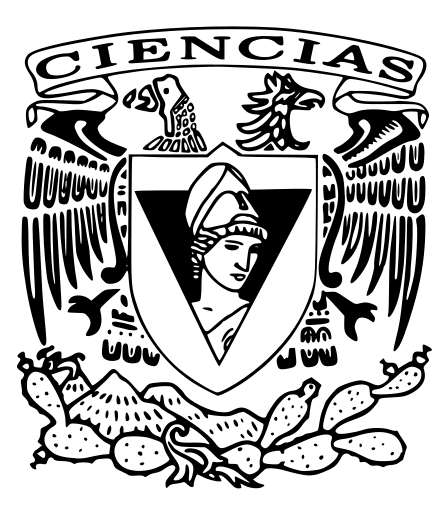
\includegraphics[scale=0.40]{1.png}	
\end{center}
\newpage
\title{\Huge Bitácora clase 8} \\
\\
Comenzamos la clase viendo algunas de las funciones de Linux, cuando un proceso se ejecuta desde la terminal queda en primer plano y la terminal ya no se puede seguir usando a menos que se abra otra, para evitar esto se debe poner la aplicación en segundo plano, para ello solo es necesario poner el signo \& después del nombre de la aplicación y así sera posible seguir usando la misma terminal. Si lo que queremos es "matar" un proceso que se esté ejecutando, basta con poner ctrl+c, o kill -9 y el proceso se detendrá en ese momento. Si solo se quiere pausar se pone el comando ctrl+z y el proceso se quedará en pausa. \\
\\
\#!/usr/bin/python2.7 se pone como comentario en python y permite ejecutar el programa directamente desde la terminal sin la necesidad de tener el shell de python, y el comentario \# -*- coding: utf-8 -*- permite poner caracteres especiales los comentarios de phython, por ejemplo acentos, diéresis, símbolos, etc.\\
\\
Una clase son todos los atributos que comparte un grupo, uno en específico es un objeto de la clase, y cada objeto es distinto aunque comparta atributos y esté relacionado con otros objetos de su misma clase. Los objetos pueden interactuar entre sí, esto es, hay interacción entre objetos de la clase y también hay interacción entre clases.\\
Nosotros interactuamos con las computadoras y podemos hacer acciones a las que les llamamos métodos, por ejemplo "pedir la palabra". Todos los de la clase tenemos atributos en común y cada uno de nosotros es diferente, pedir la palabra por medio de levantar la mano es un método que tenemos nosotros como objeto. Las acciones que realiza el objeto se llaman métodos. Hay métodos que modifican el estado de un atributo.
La notación en python es objeto.metodo no es necesario que tengan parámetros.\\
\\
También se puede ver el tipo de dato que es en python (entero, flotante) con el comando \textit{type} que te arroja qué tipo de dato es, si se pone \textit{type.\_\_name\_\_.} solo arroja el tipo directo. Se pueden covertir los enteros a flotantes con el comando \textit{float()} y  \textit{str} convierte cualquier valor numérico en una cadena. La diferencia entre función y método es que una función no depende de un objeto un método sí.\\
\\
La cadenas se pueden  sumar "Ho"+"la", y también es posible importar bibliotecas y llamarlas con un nombre más corto o cómodo para nosotros con el comando \textit{import as} y así podemos cambiar de nombre a las bibliotecas para no escribirlo todo, se puede también importar solo algunas funciones para no tener que nombrar la biblioteca antes por ejemplo importar la raíz cuadrada para no tener que poner siempre la biblioteca con el comando \textit{from math import sqrt}. Se puede incluso importar todo utilizando un \* pero no es recomendable debido a que podría traernos muchos errores después, sobretodo si lo hacemos con dos bibliotecas que manejen los mismos nombres en algunas funciones.El comando input sirva para que el programa te pregunte los valores que quieres meter sin necesidad de poner todos.



\end{document}